\begin{enumerate}[\bf 1.]
	\item 
	\item 
	\newpage
	\item 치환함수 $S:\set{0,1}^3\to\set{0,1}^3$가 다음과 같이 정의되었다고 하자.
	\begin{table}[h!]\centering\setstretch{1.5}
		\begin{tabular}{|c||c|c|c|c|c|c|c|c|}
			\hline
			$x$ & 0(000) & 1(001) & 2(010) & 3(011) & 4(100) & 5(101) & 6(110) & 7(111) \\
			\hline
			$S[x]$ & 0 & 1 & 3 & 2 & 6 & 5 & 4 & 7 \\
			\hline
		\end{tabular}
	\end{table} \\
	이 함수의 차분특성은 다음 표와 같다.
	\begin{table}[h!]\centering
		\begin{tabular}{|c|c|c|}
			\hline 
			입력차분($\alpha$) & 출력차분($\beta$) & 차분확률($P[\alpha\to\beta]$) \\ \hline
			001 & 001 & 0.5 \\
			001 & 011 & 0.5 \\
			010 & 010 & 0.5 \\
			010 & 011 & 0.5 \\
			011 & 001 & 0.5 \\
			011 & 010 & 0.5 \\
			$\vdots$ & $\vdots$ & $\vdots$ \\
			\hline
		\end{tabular}
	\end{table}
	\begin{enumerate}[(a)]
		\item 입력차분이 $\alpha=2(010)$일 때, 출력차분이 $\alpha=2(010)$가 될 확률 $P[\alpha\to\alpha]$을 구하면?
		\item 입력 마스크가 $a=5(101)$이고 출력 마스크가 $b=3(011)$일 때 \[
		NS(a,b)=\set{x\mid a\cdot x=b\cdot S[x]}
		\]의 원소의 개수는?
		\item 위에서 정의한 함수 $S:\set{0,1}^3\to\set{0,1}^3$를 사용하여 더 큰 Sbox인 $BS:s\set{0,1}^6\to\set{0,1}^6$를 다음과 같이 구성하자.
		\begin{figure}[h!]\centering
			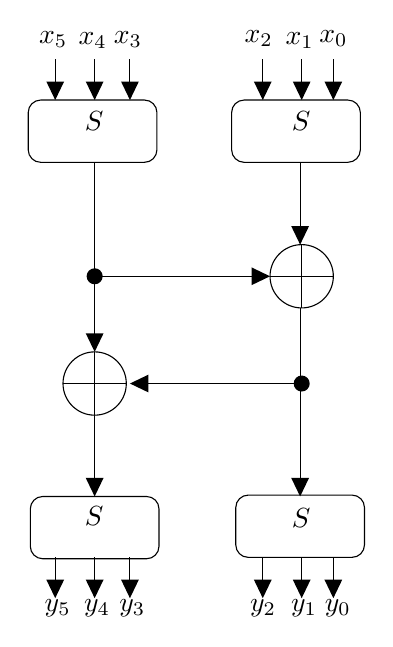
\begin{tikzpicture}[x=0.75pt,y=0.75pt,yscale=-1,xscale=1]
				%Rounded Rect [id:dp42469603179893767] 
				\draw   (280,46.67) .. controls (280,43.35) and (282.69,40.67) .. (286,40.67) -- (336,40.67) .. controls (339.31,40.67) and (342,43.35) .. (342,46.67) -- (342,64.67) .. controls (342,67.98) and (339.31,70.67) .. (336,70.67) -- (286,70.67) .. controls (282.69,70.67) and (280,67.98) .. (280,64.67) -- cycle ;
				%Rounded Rect [id:dp6966375267828862] 
				\draw   (380,237) .. controls (380,233.69) and (382.69,231) .. (386,231) -- (436,231) .. controls (439.31,231) and (442,233.69) .. (442,237) -- (442,255) .. controls (442,258.31) and (439.31,261) .. (436,261) -- (386,261) .. controls (382.69,261) and (380,258.31) .. (380,255) -- cycle ;
				%Rounded Rect [id:dp7860477123039233] 
				\draw   (281,237.67) .. controls (281,234.35) and (283.69,231.67) .. (287,231.67) -- (337,231.67) .. controls (340.31,231.67) and (343,234.35) .. (343,237.67) -- (343,255.67) .. controls (343,258.98) and (340.31,261.67) .. (337,261.67) -- (287,261.67) .. controls (283.69,261.67) and (281,258.98) .. (281,255.67) -- cycle ;
				%Rounded Rect [id:dp6309455241767805] 
				\draw   (378,46.67) .. controls (378,43.35) and (380.69,40.67) .. (384,40.67) -- (434,40.67) .. controls (437.31,40.67) and (440,43.35) .. (440,46.67) -- (440,64.67) .. controls (440,67.98) and (437.31,70.67) .. (434,70.67) -- (384,70.67) .. controls (380.69,70.67) and (378,67.98) .. (378,64.67) -- cycle ;
				%Flowchart: Or [id:dp43111622810218186] 
				\draw   (396.5,125.58) .. controls (396.5,117.16) and (403.33,110.33) .. (411.75,110.33) .. controls (420.17,110.33) and (427,117.16) .. (427,125.58) .. controls (427,134.01) and (420.17,140.83) .. (411.75,140.83) .. controls (403.33,140.83) and (396.5,134.01) .. (396.5,125.58) -- cycle ; \draw   (396.5,125.58) -- (427,125.58) ; \draw   (411.75,110.33) -- (411.75,140.83) ;
				%Flowchart: Or [id:dp07612372653447363] 
				\draw   (296.75,177.25) .. controls (296.75,168.83) and (303.58,162) .. (312,162) .. controls (320.42,162) and (327.25,168.83) .. (327.25,177.25) .. controls (327.25,185.67) and (320.42,192.5) .. (312,192.5) .. controls (303.58,192.5) and (296.75,185.67) .. (296.75,177.25) -- cycle ; \draw   (296.75,177.25) -- (327.25,177.25) ; \draw   (312,162) -- (312,192.5) ;
				%Straight Lines [id:da8522631997534107] 
				\draw    (312,70.67) -- (312,110.33) -- (312,159) ;
				\draw [shift={(312,162)}, rotate = 270] [fill={rgb, 255:red, 0; green, 0; blue, 0 }  ][line width=0.08]  [draw opacity=0] (8.93,-4.29) -- (0,0) -- (8.93,4.29) -- cycle    ;
				%Straight Lines [id:da9683498029167241] 
				\draw    (312,190) -- (312,228.67) ;
				\draw [shift={(312,231.67)}, rotate = 270] [fill={rgb, 255:red, 0; green, 0; blue, 0 }  ][line width=0.08]  [draw opacity=0] (8.93,-4.29) -- (0,0) -- (8.93,4.29) -- cycle    ;
				%Straight Lines [id:da7114989354511323] 
				\draw    (411,70.67) -- (411,107.33) ;
				\draw [shift={(411,110.33)}, rotate = 270] [fill={rgb, 255:red, 0; green, 0; blue, 0 }  ][line width=0.08]  [draw opacity=0] (8.93,-4.29) -- (0,0) -- (8.93,4.29) -- cycle    ;
				%Straight Lines [id:da028449341110133863] 
				\draw    (411,141) -- (411,228.67) ;
				\draw [shift={(411,231.67)}, rotate = 270] [fill={rgb, 255:red, 0; green, 0; blue, 0 }  ][line width=0.08]  [draw opacity=0] (8.93,-4.29) -- (0,0) -- (8.93,4.29) -- cycle    ;
				%Straight Lines [id:da37227579139782074] 
				\draw    (312,125.58) -- (393.5,125.58) ;
				\draw [shift={(396.5,125.58)}, rotate = 180] [fill={rgb, 255:red, 0; green, 0; blue, 0 }  ][line width=0.08]  [draw opacity=0] (8.93,-4.29) -- (0,0) -- (8.93,4.29) -- cycle    ;
				\draw [shift={(312,125.58)}, rotate = 0] [color={rgb, 255:red, 0; green, 0; blue, 0 }  ][fill={rgb, 255:red, 0; green, 0; blue, 0 }  ][line width=0.75]      (0, 0) circle [x radius= 3.35, y radius= 3.35]   ;
				%Straight Lines [id:da09500204271101675] 
				\draw    (411.75,177.25) -- (332,177.25) ;
				\draw [shift={(329,177.25)}, rotate = 360] [fill={rgb, 255:red, 0; green, 0; blue, 0 }  ][line width=0.08]  [draw opacity=0] (8.93,-4.29) -- (0,0) -- (8.93,4.29) -- cycle    ;
				\draw [shift={(411.75,177.25)}, rotate = 180] [color={rgb, 255:red, 0; green, 0; blue, 0 }  ][fill={rgb, 255:red, 0; green, 0; blue, 0 }  ][line width=0.75]      (0, 0) circle [x radius= 3.35, y radius= 3.35]   ;
				%Straight Lines [id:da7216603342387058] 
				\draw    (293,21) -- (293,37.67) ;
				\draw [shift={(293,40.67)}, rotate = 270] [fill={rgb, 255:red, 0; green, 0; blue, 0 }  ][line width=0.08]  [draw opacity=0] (8.93,-4.29) -- (0,0) -- (8.93,4.29) -- cycle    ;
				%Straight Lines [id:da6680400534339734] 
				\draw    (427,261) -- (427,277.67) ;
				\draw [shift={(427,280.67)}, rotate = 270] [fill={rgb, 255:red, 0; green, 0; blue, 0 }  ][line width=0.08]  [draw opacity=0] (8.93,-4.29) -- (0,0) -- (8.93,4.29) -- cycle    ;
				%Straight Lines [id:da8526371010233802] 
				\draw    (411.75,261) -- (411.75,277.67) ;
				\draw [shift={(411.75,280.67)}, rotate = 270] [fill={rgb, 255:red, 0; green, 0; blue, 0 }  ][line width=0.08]  [draw opacity=0] (8.93,-4.29) -- (0,0) -- (8.93,4.29) -- cycle    ;
				%Straight Lines [id:da6981601366843095] 
				\draw    (393,261) -- (393,277.67) ;
				\draw [shift={(393,280.67)}, rotate = 270] [fill={rgb, 255:red, 0; green, 0; blue, 0 }  ][line width=0.08]  [draw opacity=0] (8.93,-4.29) -- (0,0) -- (8.93,4.29) -- cycle    ;
				%Straight Lines [id:da5911662054724454] 
				\draw    (329,261) -- (329,277.67) ;
				\draw [shift={(329,280.67)}, rotate = 270] [fill={rgb, 255:red, 0; green, 0; blue, 0 }  ][line width=0.08]  [draw opacity=0] (8.93,-4.29) -- (0,0) -- (8.93,4.29) -- cycle    ;
				%Straight Lines [id:da3165088675709036] 
				\draw    (312,261) -- (312,277.67) ;
				\draw [shift={(312,280.67)}, rotate = 270] [fill={rgb, 255:red, 0; green, 0; blue, 0 }  ][line width=0.08]  [draw opacity=0] (8.93,-4.29) -- (0,0) -- (8.93,4.29) -- cycle    ;
				%Straight Lines [id:da34235095441645025] 
				\draw    (293,261) -- (293,277.67) ;
				\draw [shift={(293,280.67)}, rotate = 270] [fill={rgb, 255:red, 0; green, 0; blue, 0 }  ][line width=0.08]  [draw opacity=0] (8.93,-4.29) -- (0,0) -- (8.93,4.29) -- cycle    ;
				%Straight Lines [id:da9169393016789211] 
				\draw    (427,21) -- (427,37.67) ;
				\draw [shift={(427,40.67)}, rotate = 270] [fill={rgb, 255:red, 0; green, 0; blue, 0 }  ][line width=0.08]  [draw opacity=0] (8.93,-4.29) -- (0,0) -- (8.93,4.29) -- cycle    ;
				%Straight Lines [id:da7533568138302713] 
				\draw    (411.75,21) -- (411.75,37.67) ;
				\draw [shift={(411.75,40.67)}, rotate = 270] [fill={rgb, 255:red, 0; green, 0; blue, 0 }  ][line width=0.08]  [draw opacity=0] (8.93,-4.29) -- (0,0) -- (8.93,4.29) -- cycle    ;
				%Straight Lines [id:da08630039198921913] 
				\draw    (393,21) -- (393,37.67) ;
				\draw [shift={(393,40.67)}, rotate = 270] [fill={rgb, 255:red, 0; green, 0; blue, 0 }  ][line width=0.08]  [draw opacity=0] (8.93,-4.29) -- (0,0) -- (8.93,4.29) -- cycle    ;
				%Straight Lines [id:da6264691949263468] 
				\draw    (329,21) -- (329,37.67) ;
				\draw [shift={(329,40.67)}, rotate = 270] [fill={rgb, 255:red, 0; green, 0; blue, 0 }  ][line width=0.08]  [draw opacity=0] (8.93,-4.29) -- (0,0) -- (8.93,4.29) -- cycle    ;
				%Straight Lines [id:da4214884257566729] 
				\draw    (312,21) -- (312,37.67) ;
				\draw [shift={(312,40.67)}, rotate = 270] [fill={rgb, 255:red, 0; green, 0; blue, 0 }  ][line width=0.08]  [draw opacity=0] (8.93,-4.29) -- (0,0) -- (8.93,4.29) -- cycle    ;
				
				% Text Node
				\draw (405.75,236.07) node [anchor=north west][inner sep=0.75pt]    {$S$};
				% Text Node
				\draw (306,235.4) node [anchor=north west][inner sep=0.75pt]    {$S$};
				% Text Node
				\draw (405.75,45.07) node [anchor=north west][inner sep=0.75pt]    {$S$};
				% Text Node
				\draw (306,45.07) node [anchor=north west][inner sep=0.75pt]    {$S$};
				% Text Node
				\draw (284,6.4) node [anchor=north west][inner sep=0.75pt]    {$x_{5}$};
				% Text Node
				\draw (419,6.07) node [anchor=north west][inner sep=0.75pt]    {$x_{0}$};
				% Text Node
				\draw (402.75,6.73) node [anchor=north west][inner sep=0.75pt]    {$x_{1}$};
				% Text Node
				\draw (383,6.07) node [anchor=north west][inner sep=0.75pt]    {$x_{2}$};
				% Text Node
				\draw (320,6.4) node [anchor=north west][inner sep=0.75pt]    {$x_{3}$};
				% Text Node
				\draw (303,6.73) node [anchor=north west][inner sep=0.75pt]    {$x_{4}$};
				% Text Node
				\draw (286.67,280) node [anchor=north west][inner sep=0.75pt]    {$y_{5}$};
				% Text Node
				\draw (421.67,280) node [anchor=north west][inner sep=0.75pt]    {$y_{0}$};
				% Text Node
				\draw (405.42,280) node [anchor=north west][inner sep=0.75pt]    {$y_{1}$};
				% Text Node
				\draw (385.67,280) node [anchor=north west][inner sep=0.75pt]    {$y_{2}$};
				% Text Node
				\draw (322.67,280) node [anchor=north west][inner sep=0.75pt]    {$y_{3}$};
				% Text Node
				\draw (305.67,280) node [anchor=north west][inner sep=0.75pt]    {$y_{4}$};
			\end{tikzpicture}
		\end{figure}\ \\
		입력차분 $\alpha = 1(000\ 001)$에 대하여 차분확률  $P[\alpha\to\beta]$가 최대가 되는 $\beta$와 차분확률을 구하면?
	\end{enumerate}
	\begin{proof}[\sol]
		\ \begin{enumerate}[(a)]
			\item 표의 3번째 줄에 의해서 $P[\alpha\to\alpha]=P[010\to 010]=0.5$.
			\item Let $x=(x_1x_2x_3)_2$ and $S[x]=(y_3y_2y_1)_2$. Consider $a=(101)_2$ and $b=(011)_2$: \begin{figure}[h!]\centering
				\begin{tikzpicture}[>=Latex, node distance=1cm and 0cm]
					% Nodes for inputs x
					\node (x2) {\textcolor{red}{$x_2$}};
					\node (x1) [right=of x2] {{$x_1$}};
					\node (x0) [right=of x1] {\textcolor{red}{$x_0$}};
					
					% S-Box
					\node (S) [draw, minimum size=1.5cm, below=of x1, xshift=0cm] {S};
					
					% Nodes for outputs y
					\node (y2) [below=of S, xshift=-.5cm] {$y_2$};
					\node (y1) [right=of y2] {\textcolor{red}{$y_1$}};
					\node (y0) [right=of y1] {\textcolor{red}{$y_0$}};
					
					% Arrows from x to S
					\draw[->, red, line width=1.25] (x2) -- (x2|-S.north);
					\draw[->] (x1) -- (x1|-S.north);
					\draw[->, red, line width=1.25] (x0) -- (x0|-S.north);
					
					% Arrows from S to y (ensuring alignment with x_i nodes)
					\draw[->] (S.south-|x2) -- (x2|-y2.north);
					\draw[->, red, line width=1.25] (S.south-|x1) -- (x1|-y1.north);
					\draw[->, red, line width=1.25] (S.south-|x0) -- (x0|-y0.north);
				\end{tikzpicture}
			\end{figure}\ \\	
			\begin{table}[h!]\centering\renewcommand{\arraystretch}{1.5}
				\begin{tabular}{ccc|ccc|cc}
					\toprule[1.2pt]
					\textcolor{red}{$x_2$} & {$x_1$} & \textcolor{red}{$x_0$} & $y_2$ & \textcolor{red}{$y_1$} & \textcolor{red}{$y_0$} & $a\cdot x=b\cdot y$ & \\
					\hline
					0 & 0 & 0 & 0 & 0 & 0 & $0=0$ & \textcolor{green}{\checkmark}\\
					0 & 0 & 1 & 0 & 1 & 0 & $1=1$ & \textcolor{green}{\checkmark}\\
					0 & 1 & 0 & 1 & 0 & 0 & $0=0$ & \textcolor{green}{\checkmark}\\
					0 & 1 & 1 & 1 & 1 & 0 & $1=1$ & \textcolor{green}{\checkmark}\\
					1 & 0 & 0 & 1 & 0 & 1 & $1=1$ & \textcolor{green}{\checkmark}\\
					1 & 0 & 1 & 1 & 1 & 1 & $0=0$ & \textcolor{green}{\checkmark}\\
					1 & 1 & 0 & 0 & 1 & 1 & $1=0$ & \textcolor{red}{\xmark}\\
					1 & 1 & 1 & 0 & 0 & 1 & $0=1$ & \textcolor{red}{\xmark}\\
					\bottomrule[1.2pt]
				\end{tabular}
			\end{table}\\ 따라서 집합 $NS(a,b)$의 원소의 개수는 6이다.
			\item 
		\end{enumerate}
	\end{proof}
\end{enumerate}